\subsection{Rule Offload}
\label{s:offload}

\begin{figure}
\centering
%\begin{minipage}{.45\textwidth}
  \centering
  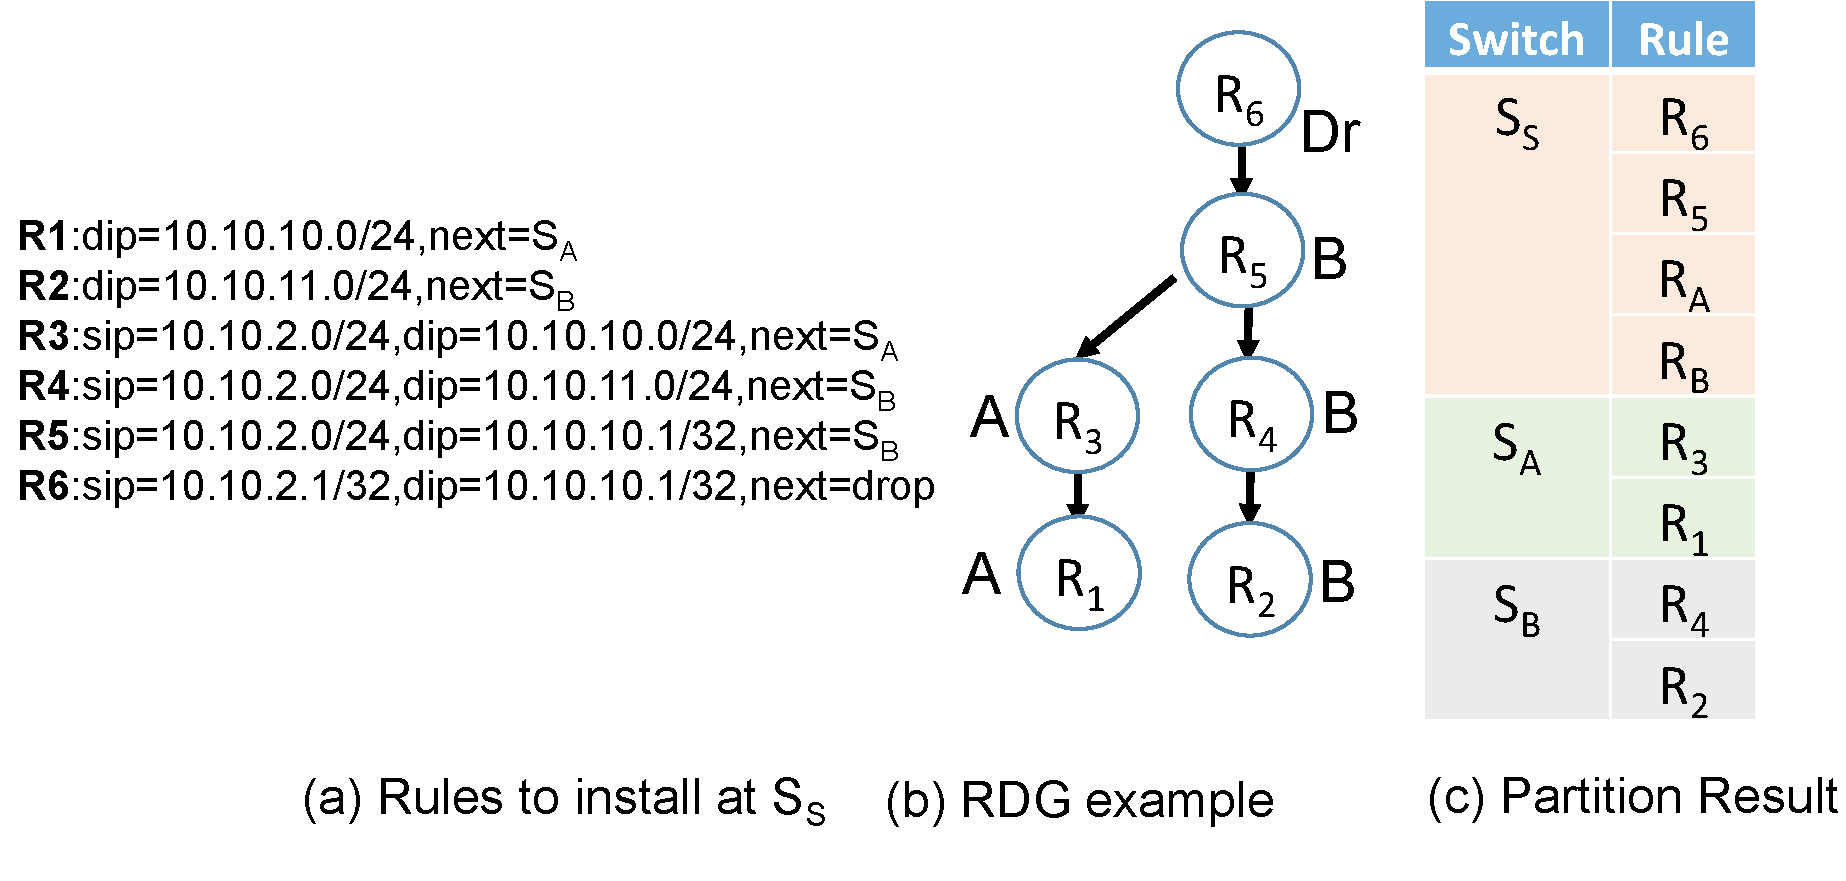
\includegraphics[width=3.0in]{figs/Rule-Offload2.pdf}
\compactcaption{Rule offloading example}
\label{fig:rule-offload}
\end{figure}

%\aditya{LI: this section does not talk about differences wrt difane, vcrib. li, can you fix?}
%\aditya{LI: we should also talk about encapsulation on the core router}

When FE selects a path for a set of flows, the same number of rules are
installed/modified in every switch along the path. Thus, a path's update
latency is determined by the switch with the largest number of existing
low priority rules (assuming \BroadcomOne), or the largest number of pending
rule installations/modifications. For example, since switch $S_S$ in
\figref{fig:flow_eng} is part of all three paths to reach switch $S_D$, a
rule must be installed in $S_S$ for every new flow, regardless of whether the
flow traverses the path through $S_A$, $S_B$, or $S_C$.  Assuming
\BroadcomOne switches, it will take at least 0.3s to install rules for 100
flows of high priority $H$ in $S_S$---the same time required to install 20
rules in $S_A$ and longer than the $\approx$0.12s required to install 40
rules in both $S_B$ and $S_C$.


%Rule offloading applies particularly to networks where tunnels are
%used, e.g., cellular networks (\S\ref{sec-motivation}), carrier networks
%that rely on label-switching, data centers using VXLAN
%%~\cite{xxx} \aditya{check this} 
%and inter-DC WAN networks such as those considered
%in~\cite{swan,b4}. In such networks, SDN applications
%control the tunnel end-points to setup overlay paths. Compared to the rate of
%changes at these tunnel end-points, the underlay, which may also be
%run using an SDN, maintains much smaller forwarding state, and
%observes much less churn in forwarding state. {\em Our approach
%  leverages these attributes of switches in the underlay to offload to
%  them rules that would otherwise be installed at the tunnel end
%  points.} 

The goal of {\em rule offloading} (\RO) is to partition rules into subsets
that can be installed at downstream switches, with the appropriate {\em
default rules} installed at upstream switches. If the original number of
rules is $N$ and no partition (together with default rules) has more than $H$
rules, then, by updating the partitions in parallel, we can reduce rule
installation latency by a factor of $\frac{N}{H}$. 

%We recursively apply RO to the switches and rules for a set of paths,
%starting the first switch(es) in the paths.
%Given a set of rules to install in a set of paths, we apply RO to the rules
%for each switch, starting from the first switch in the paths (i.e., the
%ingress switch). 
Our algorithm consists of two phases. First, given a set of rules slated for
installation in a switch $S$ (called the {\em root} switch), we partition the
rules based on their next hop, taking into account any overlap between
rules. Second, we compute default rules for each partition; these rules are
installed in the root switch to direct packets to the next hop switch where
the original rules are actually installed.

%We pick a bound $H<N$ for the number of rules to install at any switch, where 
%$N$ is the total number of rules that were slated to be installed in the
%root switch. We also choose a bound $H_{down}$ that controls the maximum
%number of rules we can offload to a switch downstream from the root switch.
%If at any iteration, partitioning at a node causes either of these bounds to
%be violated at a downstream core switch, then we terminate partitioning for
%the node. 

%The main idea in our algorithm is to recursively partition the rules into a
%number of child partitions. Since we offload to next hop switches, each
%partition has an associated next hop. Rules in
%the same partition all go to the same next hop.   
%%Actions of rules in a child partition go to the same
%%next hop. \aditya{prev sentence does not parse} 
%The partition algorithm ensures that there is no dependency among child
%partitions. For each partition, we also compute default rules to
%direct packets to that partition. The objective is to maximize the number of
%rules that can be offloaded minus the number of default rules introduced. 

\minisection{Rule Partitioning Algorithm}
%Before calculating the child partitions, 
We represent the rules to be installed at a switch as a rule dependency graph
(RDG). In an RDG, a node denotes a rule, an edge represents a dependency
between two rules, and a node label indicates a rule's action (or next hop
switch). For example, \figref{fig:rule-offload}(b) depicts the RDG for the
six rules in \figref{fig:rule-offload}(a), which are slated for installation
in switch $S_S$ in the topology in \figref{fig:flow_eng}.  Note that when
rules send packets over a tunnel, we specify the next hop in the tunnel path,
not the tunnel destination, as the node label.

%We illustrate this using an example in Figure~\ref{fig:rule-offload}. 
%Figure~\ref{fig:rule-offload}(a) shows the topology. \aaron{We don't refer to
%$S_4$ or $S_5$ anywhere, so can we just use the same topology as
%\figref{fig:flow_eng}?}  Suppose we need to 
%install six rules $R_1$, $R_2$,$\cdots$,$R_6$ to switch $S_1$. The rule 
%dependency graph is shown in Figure~\ref{fig:rule-offload}(b).
%For example, there is an edge from $R_3$ to $R_1$. This means that the two 
%rules overlap. \aaron{We need to say what the rules are, otherwise this
%example doesn't actually help the reader understand what is happening.}
%When a packet matches both rules, $R_3$ takes precedence. The labels $A$ and 
%$B$ denote the next hop of the rules' action. If a rule's action is to send 
%through a tunnel, the label will be the next hop of the tunnel path, not the 
%tunnel destination. \aaron{Can we cut out the stuff about tunnels?} 
%If a rule's action is deny, for simplicity, it will not 
%be offloaded. \aaron{Is simplicity the only reason not to do this?} 
%The pseudo code is described in Algorithm~\ref{alg:partition}. 

\begin{algorithm}
\footnotesize
\DontPrintSemicolon
% \KwData{$G$: RDG with nodes annotated with next hop label, 
%	$H$: a bound of rule count for core switches,
%	$H_{core}$: the maximum number of rules any edge switch 
%           can offload to a core switch}
% \KwResult{$P$: partition set for next hops, initially empty}
%  \tcc{traverse reverse edges}
  %$N$ = min($H$, $H\_core$)\;
%  $G'$ = reverse($G$)\; 
    \SetKw{KwIn}{in}
    \SetKw{KwOr}{or}
    \SetKw{KwAnd}{and}
    \SetKwFunction{reverseBFS}{reverseBFS}
    \SetKwFunction{isLeaf}{isLeaf}
    \SetKwFunction{ruleCount}{ruleCount}
    \SetKwFunction{children}{children}
    \ForEach{$R$ \KwIn \reverseBFS{$G$}}{
%  \tcc{$R$ is the current node}
  $i$ = label($R$)\;
  \uIf{\isLeaf{$R$}}{
	 \uIf{\ruleCount{$P_i$} $> H_{down}$ \KwOr \ruleCount{$S_i$} $>H$} {
		$P_{root}$ += $R$\;
         }
         \Else{
             $P_i$ += $R$\;
	 }
   }
%   \tcc{$R$ depends on rules with more than one distinct label}
   \Else{
       \uIf{$\forall$ \children{$R$} $\in P_i$ \KwAnd
           \ruleCount{$P_i$} $> H_{down}$ \KwAnd \ruleCount{$S_i$} $>H$} {
             $P_i$ += $R$\;
           }
         \Else{
	    	$P_{root}$ += $R$\;
	 }
   }
 }
 \caption{Rule Partition}
 \label{alg:partition}
\end{algorithm}




The algorithm (\algref{alg:partition}) performs a reverse breadth-first
traversal of the RDG. If a node $R$ is a leaf node, then it is eligible to be
placed in partition $P_i$, where $i$ is $R$'s label (or next hop). A leaf
node $R$ is placed in $P_i$ if the current number of rules in $P_i$ is less
than $H_{down}$, otherwise $R$ is placed in $P_{root}$. $H_{down}$ controls 
the maximum number of rules we can offload to a switch downstream from the root switch. If a node $R$ is not
a leaf node, then it is only placed in partition $P_i$ if all of its children
are also in partition $P_i$, and the current number of rules in $P_i$ is less
than $H_{down}$. Otherwise, $R$ is placed in $P_{root}$.
%The algorithm (\algref{alg:partition}) starts from the leaf nodes---rules 
%$R$ such that there is no $R'$ with $R \rightarrow R'$. All leaf nodes with
%the same next hop are placed in one partition. \aaron{Then what?} 
The result is an allocation of rules $R \in RDG$ to the root switch ($S$) and
its next hops.
%try to make the following simpler
\iffalse In the example, we have two next hops $S_3$ and $S_2$ through port A
and B respectively. We have two leaf rules $R_1$ and $R_2$. $R_1$'s next hop
is $S_3$ and $R_2$'s next hop is $S_2$. $R_1$ will be in partition 1 and
$R_2$ will be in partition 2. Since we have $R_3 \rightarrow R_1$ and $R_3$'s
next hop is the same as $R_1$ (which is $S_3$ through port $A$), and $R_2$
(nexthop $S_2$) and R3 have no dependency, then $R_3$ will be in partition
1.  Similarly, $R_4$ will be in partition 2. For $R_5$, $R_5 \rightarrow
R_3$, and $R_5 \rightarrow R_4$; thus, $R_5$ has to be in the root partition
(``pinned'' to the ingress switch $S_1$). Also all rules $R'$ such that $R'
\rightarrow R_5$ will be pinned down in a similar fashion. $R_6$ is such a
rule. So $R_6$ will be in the root partition.  \fi 

In the example (\figref{fig:rule-offload}), $R_1$ and $R_3$ are assigned to
partition $P_A$, $R_2$ and $R_4$ are assigned to $P_B$, and $R_5$ and $R_6$
are assigned to $P_{root}$. 
%In the example (\figref{fig:rule-offload}), $R_1$ and $R_3$ are assigned to
%partition $P_A$ and installed in switch $S_A$, $R_2$ and $R_4$ are assigned
%to $P_B$ and installed in $S_B$, and $R_5$ and $R_6$ are assigned to
%$P_{root}$ and installed in $S_S$. 
   
\iffalse
For ease of description, in the above algorithm, we do not account for switch
table occupancy or consider the detailed delay model as in
Section~\ref{s:floweng}. To accommodate table occupancy, we can stop rule
offloading process on a particular switch if the occupancy level will exceed a
threshold. To avoid high delays due to rule structure in core switches, we apply
the detailed delay model to our partition results. If the estimated delay is
higher than no offloading because of a particular core switch, we will remove
that switch from consideration and rerun the algorithm. It is also easy to
consider the delay model directly in our algorithm as we have done for flow
engineering in Section~\ref{s:floweng}. However, for simplicity, we omit the
details. 
\fi


\iffalse
\program{prog:rule-offload}
    {Recursive Rule Partition Algorithm}
{
//G: rule dependency graph with nodes annotated with next hop label \\
//$\mathcal{P}_i$: partition $i$ for next hop $i$, initially empty \\
//$C_i$: set of rules covering the flowspace of partition $i$ \\
//$N$: threshold for extra covering rules  \\
While (BFS from leaf node) \{ //traverse reverse edges\\
\> If rule $R_i$ with label $L_i$ depends on no other rules, \\
\>\>\> include $R_i$ in $\mathcal{P}_{L_i}$\\ 
\> Else If rule $R_i$ depends on rules with more than one distinct label \\
\>\>\> pin the rule to the root partition \\
\> Else \\ 
\>\>\> If rule $R_i$ results in $n>N$ covering rules, \\
\>\>\>\>\>\>    skip $R_i$ \\
\>\>\> Else     include $R_i$ in $\mathcal{P}_{L_i}$\\ 
\} \\
}
\fi



\minisection{Computing Default Rules} 
Given the partitions for the next hop switches, we must compute a set of
default rules that {\em cover} the rules in each partition. These default
rules are added to $P_{root}$ to forward packets to the appropriate next hop
switch, where the rules in each partition (excluding $P_{root}$) are 
installed.
%Given two partitions A and B computed above, we wish determine default rules
%that need to go into A and B's root partition. 
The main challenge is dealing with the fact that the intersection of default
rules may include rules from multiple partitions. 
%This introduces ambiguity at the root. 
Splitting the default rules into smaller rules can address this, but we must
be careful not to introduce too may default rules and undo the benefits of
RO.
%We present a heuristic optimization, described briefly below.

Our heuristic from computing default rules is shown in
\algref{alg:default_rule}. Given the rules in a pair of partitions $P_i$ and
$P_j$, we create a {\em covering rectangle} for the rules in each partition,
denoted as $C_i$ and $C_j$. A covering rectangle is one whose source IP range
covers the entire source IP range specified in the rules in a partition;
likewise for destination IPs. This can easily be extended to higher
dimensions if rules are based on more than just source and destination IPs.
%For simplicity, we assume that each rule can be
%represented by a rectangle (src IP, dst IP). Our heuristic easily be extended
%to higher dimensions.

If the number of rules from either $P_i$ or $P_j$ in $C_i \cap C_j$ is below
a threshold $\Theta$, then all such rules are ``promoted'' to the root
partition $P_{root}$. We also create two default rules, one each for
$C_i$ and $C_j$, and install them in the root switch $S$.

If, however, the number of rules in $C_i \cap C_j$ exceeds $\Theta$, then we
further divide both $C_i$ and $C_j$ into two sub-rectangles, and we repeat
the process above for pairs of sub-rectangles, one from each partition.
We recursively repeat the process for a small number of steps. If at the
end of these steps, the combined number of default rules and rules in
$P_{root}$ is significant ($> \Omega$), then we merge $P_i$ and $P_j$ and
simply install all of their rules at the root switch $S$.


%\fi

\begin{algorithm}
\footnotesize
\SetKwFunction{defaultRule}{defaultRule}
\DontPrintSemicolon
% \KwData{rule partition set $P$}
% \KwResult{default rules at root and new partition set $P$}
  \SetKwFunction{proc}{checkOverlap}
    \SetKw{KwIn}{in}
    \SetKwFunction{ruleCount}{ruleCount}
%  $P'$ = $P$ - $P_{root}$\;
 \ForEach{distinct partition pair $(P_i, P_j)$ \KwIn $P$}{
  get covering rectangles $C_i$ and $C_j$ for $P_i$ and $P_j$\;
  \proc{$P$, $C_i$, $C_j$}\;
  }
  \SetKwProg{myproc}{Procedure}{}{}
  \myproc{\proc{$P$, $C_i$, $C_j$}} { 
  \uIf{\ruleCount{$C_i$ $\cap$ $C_j$} $\geq$ $\Theta$} {
   	divide $C_i$ and $C_j$ into two sub-rectangles each\;
	\ForEach{sub-rectangle pair ($C'_i$, $C'_j$)}{
		\proc{$P$, $C'_i$, $C'_j$}\;
	}
	
   }
   \Else{
        move $C_i$ $\cap$ $C_j$ to $P_{root}$\;
	$P_{root}$ += \defaultRule{$P_i$, $C_i$}\;
	$P_{root}$ += \defaultRule{$P_j$, $C_j$}\;
   }
  }
 \caption{Computing default rules}
 \label{alg:default_rule}
\end{algorithm}




%In the example,  we have two next hops $S_3$ and $S_2$ through port A and B
%respectively. $R_1$ will be in partition 1 and $R_2$ will be in partition 2.
%Since we have $R_3 \rightarrow R_1$ and $R_3$'s next hop is the same as
%$R_1$, then $R_3$ will be in partition 1. Similarly, $R_4$ will be in
%partition 2. $R_5$ has to be in the root partition becase it has
%dependencies.  Also all rules $R'$ such that $R' \rightarrow R_5$ will be
%pinned down in a similar fashion. $R_6$ is such a rule. So $R_6$ will be in
%the root partition.  Because we need to direct traffic to the appropriate
%next hop for offloading, we need to create default rules to cover the
%flowspace of the partitions (we will explain later).  Suppose one rule $R_A$
%covers the flowspace of partition 1 and one rule $R_B$ covers the flowspace
%of partition 2. The final rules to install at switches $S_1,S_2,S_3$ is shown
%in Figure~\ref{fig:rule-offload}(c). Four rules will be installed in switch
%$S_1$ and two each will be installed at switches $S_2,S_3$ respectively. This
%reduces the number of rules to install at switch $R_1$ by one third.

%We recursively apply RO to the switches and rules for a set of paths,
%starting the first switch(es) in the paths.
%Given a set of rules to install in a set of paths, we apply RO to the rules
%for each switch, starting from the first switch in the paths (i.e., the
%ingress switch). 

We recursively apply RO to the switches in a set of paths, starting at the
ingress switch for the paths (e.g., $S_S$ in \figref{fig:flow_eng}),
followed by the second switch in each path, and so on.
%We then run the above routine recursively starting at the edge switch,
%followed by running it at the next hop core switches over the rules
%allocated to them, and so on. \aaron{Does each switch have its own RDG?} 
The termination condition is that a set number of hops in each path are
explored. If at termination, the number of rules accommodated at every
switch, except the ingress switch, is $<H$, then we lower $H$ by a factor
$\gamma < 1$ and repeat again. If $H^*$ is the value of $H$ at the last of
such iterations, then we achieve a speedup of $\frac{N}{H^*}$ from installing
the offloaded rules in parallel. When running RO for an entire network, we
sort ingress switches in decreasing order of the number of rules to be 
installed and apply RO in this order. 
For simplicity, we have assumed that all the switches have the same latency
model; to accommodate switch diversity, we can assign different cost for the
rules offloaded to different core switches.

%The time complexity of the algorithm is based on the
%RDG: $\mathcal{O}$($\abs{V}$+$\abs{E}$). \aaron{Is this to run for a single
%switch?}
%, where $V$ and $E$ are the vertex and edges of rule dependency graph $G$. 


